\documentclass[tikz,12pt]{standalone}
\usepackage{textcomp}

\usepackage{tikz}
\usetikzlibrary{shapes.geometric, arrows}
\usepackage{xcolor}

% Custom colors
\definecolor{backcolour}{rgb}{0.95,0.95,0.92}
\definecolor{backcolour}{RGB}{229, 229, 229}
% Polar Night Palette
\definecolor{nightDarkest}{RGB}{46, 52, 64}
\definecolor{nightDark}{RGB}{59, 66, 82}
\definecolor{nightMid}{RGB}{67, 76, 94}
\definecolor{nightLight}{RGB}{76, 86, 106}
% Snow Storm Palette
\definecolor{snowDark}{RGB}{216, 222, 233}
\definecolor{snowMid}{RGB}{229, 233, 240}
\definecolor{snowLight}{RGB}{236, 239, 244}
% Frost Palette
\definecolor{frostTurqoise}{RGB}{143, 188, 187}
\definecolor{frostLightBlue}{RGB}{136, 192, 208}
\definecolor{frostMidBlue}{RGB}{129, 161, 193}
\definecolor{frostDarkBlue}{RGB}{94, 129, 172}
% Aurora Palette
\definecolor{auroraLila}{RGB}{180, 142, 173}
\definecolor{auroraRed}{RGB}{191, 97, 106}
\definecolor{auroraOrange}{RGB}{208, 135, 112}
\definecolor{auroraYellow}{RGB}{235, 203, 139}
\definecolor{auroraGreen}{RGB}{163, 190, 140}

% Baskervald X for roman, with oldstyle figure
\usepackage[osf]{Baskervaldx}
% load amssymb before newtxmath to avoid problem with \Bbbk
\usepackage{amssymb}
% Nice math calligraphic font 
\usepackage[cal=boondoxo]{mathalpha}
% Math font to match
\usepackage[bigdelims,baskervaldx]{newtxmath}

% \usetikzlibrary{backgrounds}

\begin{document}


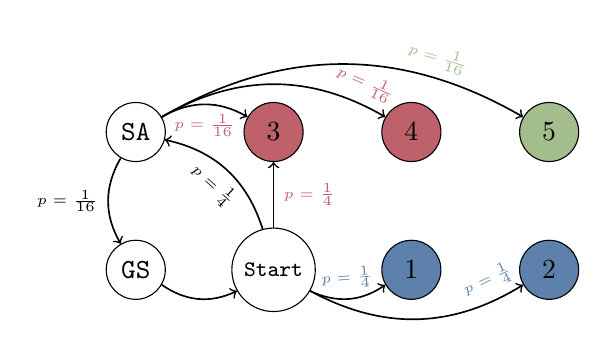
\begin{tikzpicture}
    [
		% show background rectangle,
		node distance=1.75cm,
		place/.style={
			draw, circle, align=center, minimum size=0.75cm, fill=white
		}
	]

% \draw [use as bounding box]
	% (left, down) - (right, up)
	% (-1.2cm, -2.45cm) rectangle (5.65cm, 1.15cm);

% Nodes
\node (RA) [place, align=center] {\ttfamily SA};
\node (three) [place, right of=RA, fill=auroraRed] {3};
\node (four) [place, right of=three, fill=auroraRed] {4};
\node (five) [place, right of=four, fill=auroraGreen] {5};
\node (GS) [place, below of=RA] {\ttfamily GS};
\node (start) [place, right of=GS] {\ttfamily\footnotesize Start};
\node (one) [place, right of=start, fill=frostDarkBlue] {1};
\node (two) [place, right of=one, fill=frostDarkBlue] {2};

% Transitions
% \draw [->, semithick, bend left]
% 	(start) to node [auto]
% 	{\tiny $p=\frac{1}{4}$} (RA) {};

% \draw [->, , bend right] (start) to (GS) {};
\draw [->, semithick, bend right]
	(start) to node [sloped, auto]
	{\tiny \color{frostDarkBlue}{$p=\frac{1}{4}$}} (one) {};

\draw [->, semithick, bend right]
	(start) to node [sloped, auto, very near end]
	{\tiny \color{frostDarkBlue}{$p=\frac{1}{4}$}} (two) {};

\draw [->, semithick]
	(start) to node [auto, swap]
	{\color{auroraRed}{\tiny $p=\frac{1}{4}$}} (three);

% \draw [->, semithick, in=225]
% 	(start) to node [sloped, auto, near end]
% 	{\tiny $p=\frac{1}{4}$} (four);

% \draw [->, semithick, in=250]
% 	(start) to node [sloped, auto, near end]
% 	{\tiny $p=\frac{1}{4}$} (five);

\draw [->, semithick, bend left]
	(RA) to node [auto, sloped, swap]
	{\color{auroraRed}{\tiny$p=\frac{1}{16}$}} (three) {};

\draw [->, semithick, bend left]
	(RA) to node [auto, sloped, very near end]
	{\color{auroraRed}{\tiny$p=\frac{1}{16}$}} (four) {};

\draw [->, semithick,bend left]
	(RA) to node [auto, sloped, near end, outer ysep=0]
	{\color{auroraGreen}{\tiny$p=\frac{1}{16}$}} (five) {};

\draw [->, semithick, bend right]
	(start) to node [auto, sloped, swap]
	{\tiny$p=\frac{1}{4}$} (RA) {};

\draw [->, semithick, bend right]
	(RA) to node [auto, swap]
	{\tiny$p=\frac{1}{16}$} (GS) {};

\draw [->, semithick, bend right]
	(GS) to node [auto, swap]
	{} (start) {};

\end{tikzpicture}

\end{document}
